\section{Additional Experiment Results}  \label{sec:appendix-more-experiments}


% \textbf{Reaction loss coefficient $\lambda_{\text{react}}$}. Table \ref{tab:ablation_coef} shows that increasing the reaction loss coefficient $\lambda_{\text{react}}$ from a small value (0.01) to a moderate range (0.05--0.1) consistently improves both visual quality and reaction-related metrics, indicating that stronger supervision helps the model learn more accurate and temporally aligned behaviors. However, further increasing $\lambda_{\text{react}}$ (e.g., $\geq$ 0.2) leads to degraded performance in both generation quality and reaction accuracy, suggesting that overly strong supervision disrupts the balance between the two objectives. Overall, $\lambda_{\text{react}}$=0.05 achieves the best trade-off across metrics.

% \begin{table}[t]
%     \centering
%     \fontsize{7.5pt}{6.8pt}\selectfont
%     \setcellgapes{1.5pt}
%     \makegapedcells
%     \setlength{\tabcolsep}{2pt}
%     \caption{Ablation study on the coefficient of the temporal reaction loss.}
%     \label{tab:ablation_coef}
%     \begin{tabular}{c|cccccccc|cccc}
%         \Xhline{1.2pt}
        
%         \multirow{2}{*}{\makecell[c]{Reaction\\Loss Coef.}} 
%         & \multicolumn{12}{c}{Metrics} \\
        
%         \cline{2-13}
        
%         & PSNR $\uparrow$
%         & SSIM $\uparrow$
%         & FID $\downarrow$
%         & FVD $\downarrow$
%         & Var $\uparrow$
%         & LPIPS $\downarrow$
%         & rPCC $\downarrow$
%         & DI-Sync $\uparrow$
%         & R-F1 $\uparrow$
%         & R-tIoU $\uparrow$
%         & R-ATD $\downarrow$
%         & R-FID $\downarrow$ \\
        
%         \hline
        
%         0.01 
%         & 15.446 & 0.573 & 37.034 & 178.878 & 1.848 & 0.502 
%         & 0.232 & 0.196 & 0.572 & 0.606 & 78.672 & 17.976 \\
        
%         \textbf{0.05} 
%         & \textbf{17.973} & 0.601 & \textbf{35.691} & \textbf{142.456} & \textbf{2.913} & \smash{\uline{0.454}} 
%         & \textbf{0.227} & \textbf{0.245} & 0.594 & \smash{\uline{0.704}} & \textbf{57.386} & \textbf{15.192} \\
        
%         0.1 
%         & 17.904 & \textbf{0.632} & 36.147 & \smash{\uline{144.895}} & \smash{\uline{2.901}} & \textbf{0.447} 
%         & \smash{\uline{0.230}} & 0.223 & \textbf{0.613} & \textbf{0.711} & \smash{\uline{64.790}} & 16.326 \\
        
%         0.2 
%         & \smash{\uline{17.566}} & \smash{\uline{0.610}} & \smash{\uline{36.032}} & 149.286 & 2.744 & 0.471 
%         & 0.245 & \smash{\uline{0.230}} & \smash{\uline{0.602}} & 0.684 & 69.131 & 15.875 \\
        
%         0.5 
%         & 15.297 & 0.595 & 39.115 & 163.477 & 2.331 & 0.502 
%         & 0.248 & 0.205 & 0.582 & 0.695 & 77.437 & \smash{\uline{15.548}} \\
        
%         1 
%         & 15.132 & 0.560 & 42.855 & 169.964 & 1.948 & 0.545 
%         & 0.261 & 0.210 & 0.549 & 0.663 & 78.551 & 17.036 \\
        
%         \Xhline{1.2pt}
%     \end{tabular}
% \end{table}






\subsection{Qualitative Results on Seamless Dataset}  \label{sec:appendix-seamless}

\begin{figure}[t]
    \centering
    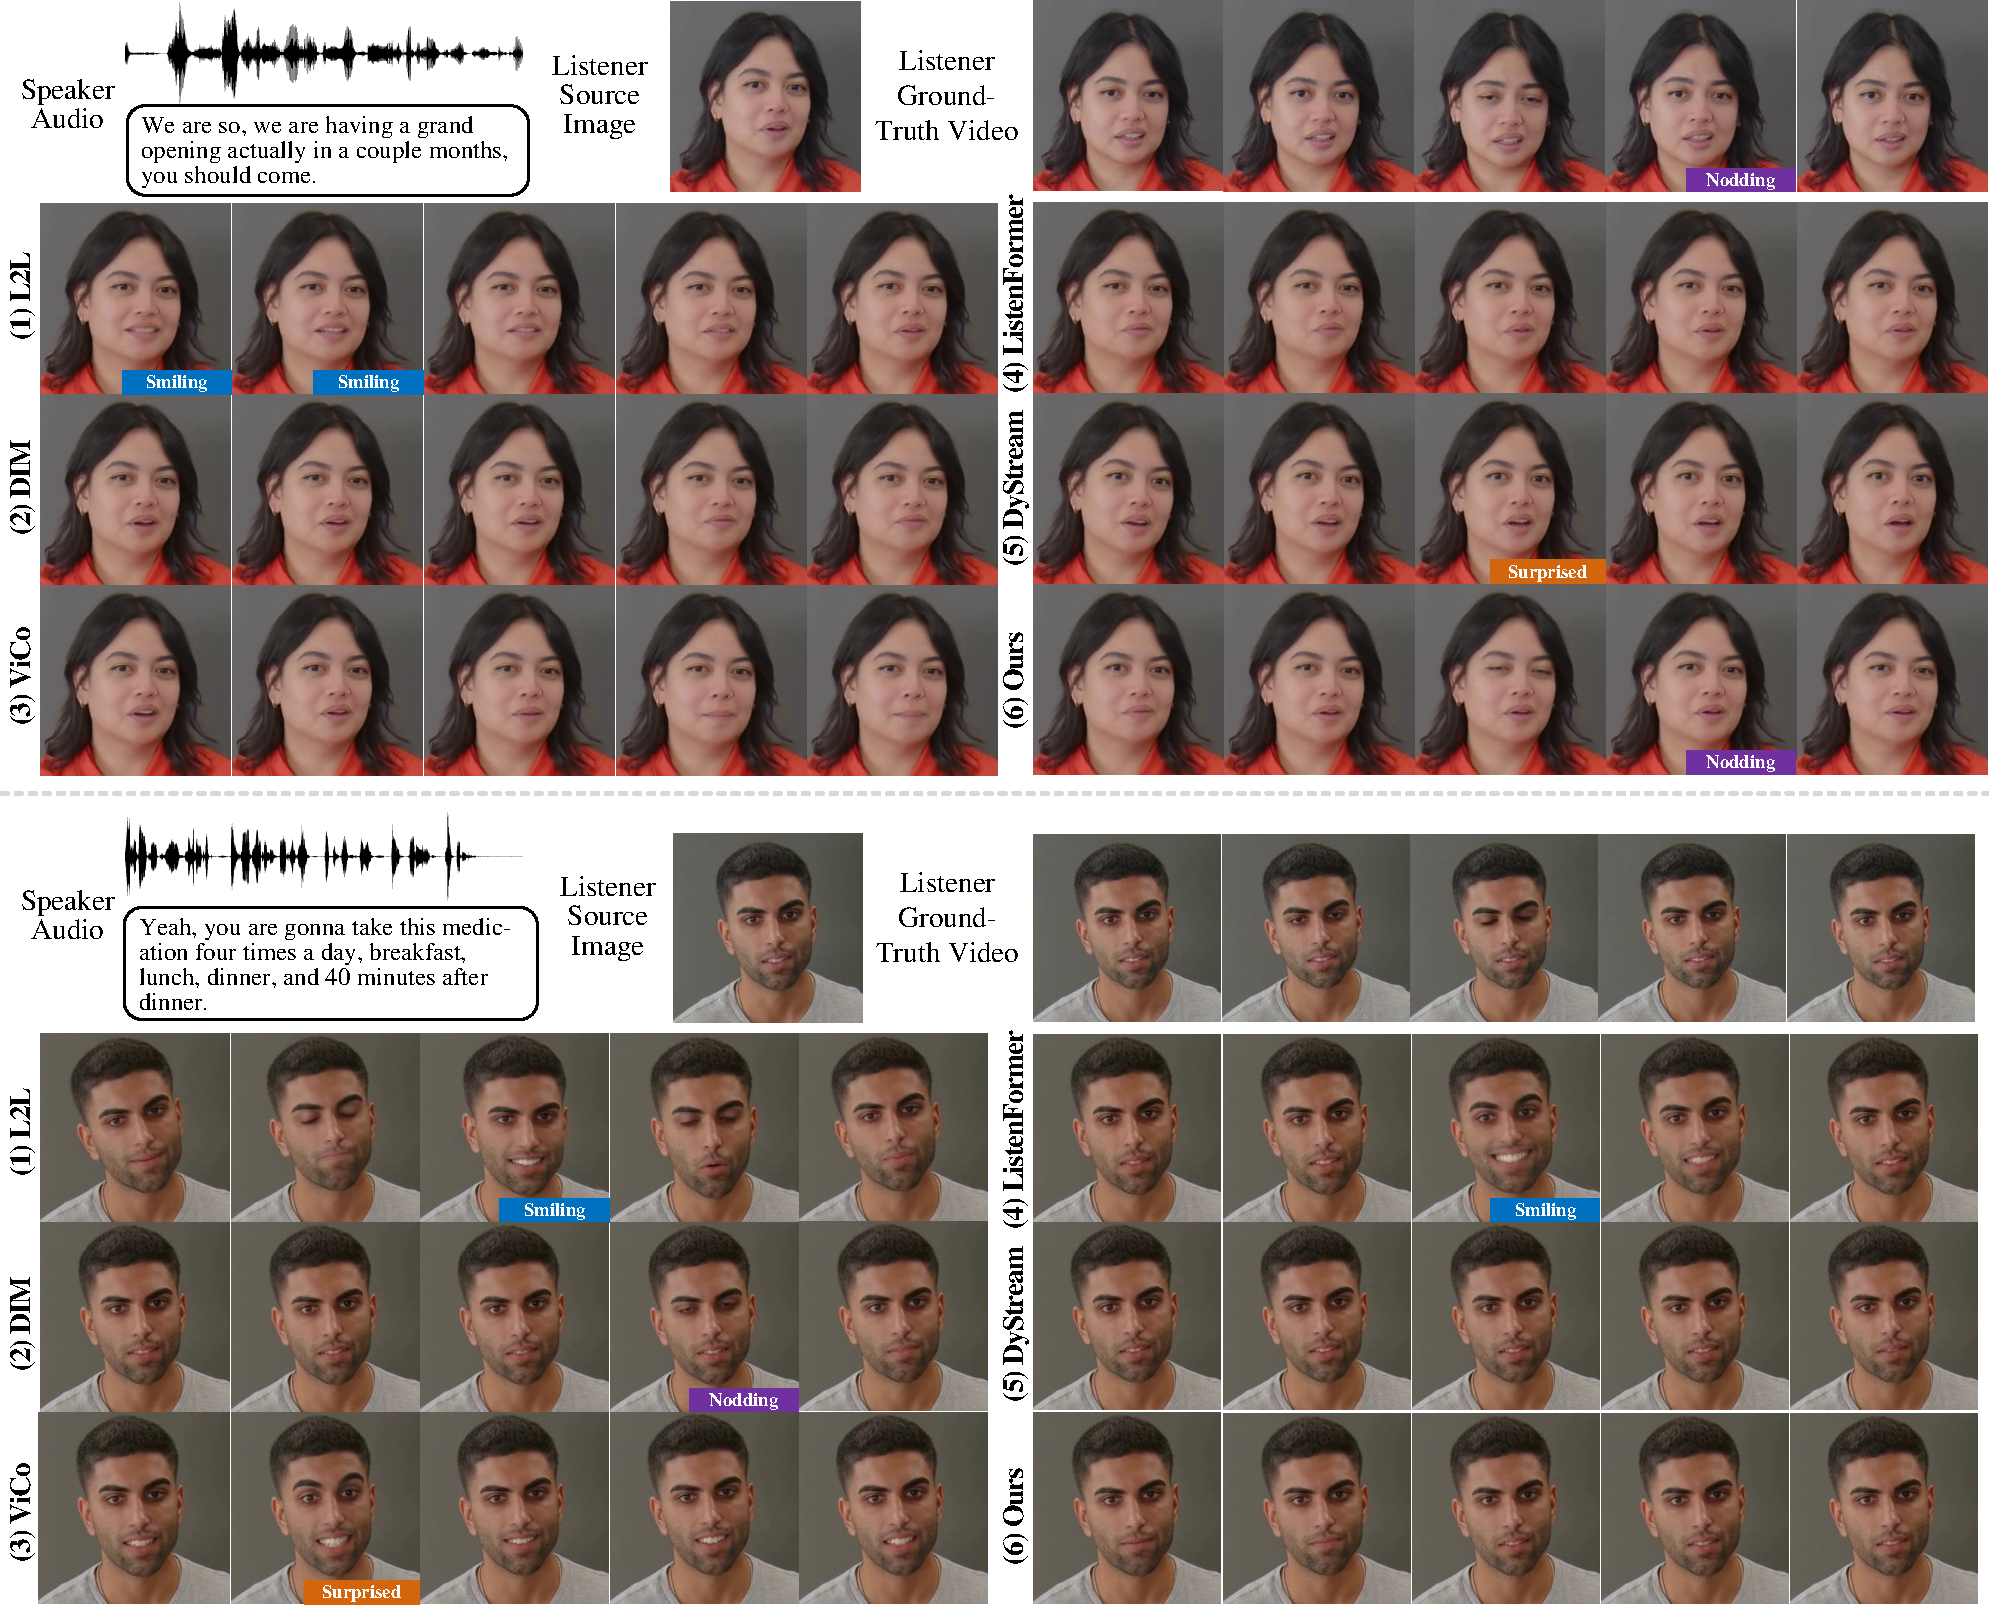
\includegraphics[width=\linewidth,keepaspectratio]{files/result_seamless.pdf}
    \caption{Qualitative comparisons between our baseline and other state-of-the-art methods on Seamless dataset. Reaction labels are displayed when a reaction is detected at the corresponding frame. Our method generates more natural listening motions and reactions that are more temporally aligned with ground truths than other comparisons.}
    \label{fig:seamless}
\end{figure}

Fig. \ref{fig:seamless} presents additional qualitative comparisons on the Seamless dataset, illustrating both the realism and temporal alignment of generated listener behaviors. We show two representative conversational scenarios with different speakers and listener identities.

Similar to observations illustrated in Fig. \ref{fig:realtalk} for RealTalk, clear differences can be seen that the comparison methods often produce overly static or weak facial dynamics, with limited variation across frames. As a result, these methods frequently fail to trigger meaningful listener reactions even when strong conversational cues are present in the speaker audio. Most importantly, they sometimes output reactions that are relatively not so appropriate or closely associated with the given contexts.

Our method, on the other hand, produces more expressive and contextually appropriate listener behaviors. In the first example, where the speaker exhibits a clear emphasis in speech, our model generates a well-timed nodding response that closely aligns with the ground-truth reaction, while other methods either miss the reaction or produce weaker and less consistent motion. In the second example, our method captures a subtle smiling response that emerges naturally along the conversational flow, whereas competing methods either delay the response or generate less coherent facial expressions. Notably, our reactions are not only more visible, but also better synchronized with the speaker’s prosodic cues.

Overall, these qualitative results demonstrate that our approach improves both the \textit{type correctness} and \textit{temporal alignment} of listener reactions, leading to more natural, expressive, and coherent conversational behaviors compared to prior methods.








\subsection{More Ablation Studies}  \label{sec:appendix-ablation}

Due to space limit in the main paper, here we present three more ablation studies, including input speaker audio length, prosody channel projection, and temporal reaction loss type.


\textbf{Input speaker audio length}. Different length of input audio from speaker can provide different amount of contexts. Table \ref{tab:audio_length} shows that increasing speaker's audio length generally improves performance, as longer temporal context provides richer cues for both motion generation and reaction prediction. Performance improves notably from 2s to 10s across most metrics, including visual quality (PSNR, FVD) and reaction accuracy (DI-Sync, R-F1, R-tIoU). However, further increasing the length (e.g., 20s or 50s) brings marginal gains or even slight degradation, likely due to increased temporal redundancy and modeling difficulty. Overall, 10s achieves the best balance between sufficient context and stable modeling.

\begin{table}[t]
    \centering
    \fontsize{7.5pt}{7pt}\selectfont
    \setcellgapes{1.5pt}
    \makegapedcells
    \setlength{\tabcolsep}{2pt}
    \caption{Effect of audio length on model performance.}
    \label{tab:audio_length}
    \begin{tabular}{c|cccccccc|cccc}
        \Xhline{1.2pt}
        
        \multirow{2}{*}{\makecell[c]{Audio\\Length (s)}} 
        & \multicolumn{12}{c}{Metrics} \\
        
        \cline{2-13}
        
        & PSNR $\uparrow$
        & SSIM $\uparrow$
        & FID $\downarrow$
        & FVD $\downarrow$
        & Var $\uparrow$
        & LPIPS $\downarrow$
        & rPCC $\downarrow$
        & DI-Sync $\uparrow$
        & R-F1 $\uparrow$
        & R-tIoU $\uparrow$
        & R-ATD $\downarrow$
        & R-FID $\downarrow$ \\
        
        \hline
        
        2 
        & 16.684 & 0.584 & 37.780 & 164.74 & 2.686 & 0.496 
        & \smash{\uline{0.212}} & 0.224 & 0.577 & 0.678 & 68.697 & 17.126 \\
        
        3 
        & 16.987 & 0.592 & 36.158 & 152.08 & 2.874 & 0.492 
        & 0.236 & \smash{\uline{0.242}} & 0.588 & 0.684 & 64.563 & 16.554 \\
        
        5 
        & 17.371 & \smash{\uline{0.599}} & \smash{\uline{35.796}} & \smash{\uline{144.32}} & \textbf{2.952} & 0.466 
        & \textbf{0.201} & 0.237 & \textbf{0.596} & 0.695 & 60.285 & \smash{\uline{15.724}} \\
        
        \textbf{10} 
        & \textbf{17.973} & \textbf{0.601} & \textbf{35.691} & \textbf{142.456} & 2.913 & 0.454 
        & 0.227 & \textbf{0.245} & \smash{\uline{0.594}} & \smash{\uline{0.704}} & \textbf{57.386} & \textbf{15.192} \\
        
        20 
        & \smash{\uline{17.884}} & 0.597 & 35.824 & 147.67 & \smash{\uline{2.949}} & \textbf{0.444} 
        & 0.233 & 0.240 & 0.590 & \textbf{0.712} & \smash{\uline{58.597}} & 16.055 \\
        
        50 
        & 17.592 & 0.589 & 36.319 & 145.34 & 2.940 & \smash{\uline{0.449}} 
        & 0.248 & 0.235 & 0.592 & \smash{\uline{0.707}} & 62.446 & 15.893 \\
        
        \Xhline{1.2pt}
    \end{tabular}
\end{table}



\textbf{Prosody Channel Projection}. In our architecture, we project the channel dimension from 1 of frame-aligned prosodic intensity scalar $p$ into 4 of prosody condition $w_{\tilde{p}}$. We ablate this channel projection in Table \ref{tab:prosody_channels}. The results show that introducing a learnable channel projection for the prosodic intensity signal consistently improves performance compared to using the raw scalar (channel=1), indicating the benefit of increasing representation capacity for prosody conditioning. As the channel dimension increases from 1 to 4, we observe steady gains in both generation quality (e.g., lower FVD, LPIPS, and rPCC) and reaction-related metrics (e.g., higher R-tIoU and lower R-ATD), suggesting improved temporal alignment and more accurate reaction dynamics. However, further increasing the channel dimension to 8 does not bring consistent improvements and slightly degrades several metrics, implying diminishing returns and potential over-parameterization. Overall, projecting the prosodic signal to a moderate channel size (4) achieves the best trade-off between expressiveness and stability, and is thus adopted in our final model.

\begin{table}[t]
    \centering
    \fontsize{7.5pt}{7pt}\selectfont
    \setcellgapes{1.5pt}
    \makegapedcells
    \setlength{\tabcolsep}{2pt}
    \caption{Ablation study on channel dimension projection for prosodic condition.}
    \label{tab:prosody_channels}
    \begin{tabular}{c|cccccccc|cccc}
        \Xhline{1.2pt}
        
        \multirow{2}{*}{\makecell[c]{Channel\\number}} 
        & \multicolumn{12}{c}{Metrics} \\
        
        \cline{2-13}
        & PSNR $\uparrow$
        & SSIM $\uparrow$
        & FID $\downarrow$
        & FVD $\downarrow$
        & Var $\uparrow$
        & LPIPS $\downarrow$
        & rPCC $\downarrow$
        & DI-Sync $\uparrow$
        & R-F1 $\uparrow$
        & R-tIoU $\uparrow$
        & R-ATD $\downarrow$
        & R-FID $\downarrow$ \\
        
        \hline
        1 
        & 17.797 & 0.596 & \smash{\uline{35.704}} & 148.925 & 2.783 & 0.475 
        & 0.235 & 0.242 & \textbf{0.602} & 0.689 & 70.474 & 16.345 \\
        
        2 
        & 18.021 & \textbf{0.603} & 35.832 & \smash{\uline{144.796}} & \textbf{2.928} & \smash{\uline{0.457}} 
        & 0.234 & 0.233 & 0.582 & 0.695 & 60.178 & 16.502 \\
        
        \textbf{4} 
        & 17.973 & \smash{\uline{0.601}} & \textbf{35.691} & \textbf{142.456} & \smash{\uline{2.913}} & \textbf{0.454} 
        & \smash{\uline{0.227}} & 0.245 & \smash{\uline{0.594}} & \textbf{0.704} & \textbf{57.386} & \textbf{15.192} \\
        
        8 
        & \textbf{18.792} & 0.584 & 35.989 & 145.776 & 2.862 & 0.460 
        & 0.230 & \smash{\uline{0.247}} & 0.582 & \smash{\uline{0.699}} & \smash{\uline{59.404}} & \smash{\uline{15.220}} \\
        
        16 
        & \smash{\uline{18.464}} & 0.581 & 35.794 & 146.435 & 2.848 & \smash{\uline{0.457}} 
        & \textbf{0.211} & \textbf{0.250} & 0.556 & \textbf{0.704} & 58.691 & 15.348 \\
        \Xhline{1.2pt}
    \end{tabular}
\end{table}







\begin{table}[!htbp]
    \centering
    \fontsize{7.5pt}{7pt}\selectfont
    \setcellgapes{1.5pt}
    \makegapedcells
    \setlength{\tabcolsep}{2pt}
    \caption{Ablation study on reaction loss type.}
    \label{tab:reaction_loss}
    \begin{tabular}{c|cccccccc|cccc}
        \Xhline{1.2pt}
        
        \multirow{2}{*}{\makecell[c]{Channel\\number}} 
        & \multicolumn{12}{c}{Metrics} \\
        
        \cline{2-13}
        & PSNR $\uparrow$
        & SSIM $\uparrow$
        & FID $\downarrow$
        & FVD $\downarrow$
        & Var $\uparrow$
        & LPIPS $\downarrow$
        & rPCC $\downarrow$
        & DI-Sync $\uparrow$
        & R-F1 $\uparrow$
        & R-tIoU $\uparrow$
        & R-ATD $\downarrow$
        & R-FID $\downarrow$ \\
        
        \hline
        BCE
        & 17.695 & 0.597 & 35.702 & 159.266 & 2.884 & 0.461 
        & 0.240 & \textbf{0.249} & \textbf{0.598} & \textbf{0.712} & 59.185 & 17.996 \\
        
        Smooth L1 
        & \textbf{17.973} & \textbf{0.601} & \textbf{35.691} & \textbf{142.454} & \textbf{2.913} & \textbf{0.454} 
        & \textbf{0.227} & 0.245 & 0.594 & 0.704 & \textbf{57.386} & \textbf{15.192} \\

        \Xhline{1.2pt}
    \end{tabular}
\end{table}

\textbf{Reaction Loss Type}. We use Smooth-L1 for computing the reaction loss, and we ablate this loss function with BCE loss, where results are reported in Table \ref{tab:reaction_loss}. While BCE achieves slightly better scores on detection-oriented metrics such as DI-Sync, R-F1, and R-tIoU, Smooth-L1 improves generation quality (e.g., lower FVD, LPIPS, and rPCC) as well as temporal deviation metrics (R-ATD and R-FID). This suggests that Smooth-L1 provides a more stable and regression-friendly supervision signal for continuous frame-wise reaction intensities, leading to better temporal consistency and overall motion quality. Therefore, we adopt Smooth-L1 as the default reaction loss.